\chapter{反射音方向分布特性}

\section{方向情報を含む物理指標}

\section{反射音の方向情報}
反射音の方向情報をみるため、解析で得られたインパルス応答から鉛直方向成分、側方成分、前後方向成分に分解した。なお、反射音の到来角度は音源方向を$0^\circ$とした。
\\ 初期反射音($t$=0$\sim$80[ms])の側方成分は観測高さによる違いは見られないものの、鉛直方向成分は座席面遠方音場($H$=14.0)において豊富に到来しているのに対し、座席面近傍音場($H$=1.2)では著しく不足していることが読み取れる。

\includepdf[pages=-, angle=90]{05_att/ir_rec3.pdf}

\section{反射音方向別エネルギ比}
ここで、反射音の到来方向バランスを定量的に把握するため、初期反射音の全エネルギ($t$=0$\sim$80[ms])に対する鉛直方向成分の割合$ER_V$(vertical energy ratio)、側方成分の割合$ER_L$(lateral energy ratio)、前後方向成分の割合$ER_G$(longitudinal energy ratio)を各々算出した(\textbf{式}\ref{eq:ERV}$\sim$\ref{eq:ERG})。ここで$\delta$は仰角(鉛直上方向:0$^\circ$)、$\theta$は水平角(側方:0$^\circ$)を表す。
観測高さ$H$ごとの反射音方向別エネルギ比の分布を\figref{sankaku14}$\sim$\figref{sankaku1}に示す。
観測高さが高くなるにつれ、$ER_V$の増加と$ER_G$の減少により、各方向成分が均等に到達する点($\frac{1}{3},\frac{1}{3},\frac{1}{3}$)に分布が集中している。

\begin{table}[htbp]
\begin{equation}
  \label{eq:ERV}
  ER_V = {\frac{\displaystyle\int_0^{80}p^2(t)cos^2{\delta}dt}{\displaystyle\int_0^{80}p^2(t)dt}} 
\end{equation}

\begin{equation}
  \label{eq:ERL}
  ER_L = {\frac{\displaystyle\int_0^{80}p^2(t)sin^2{\delta}cos^2{\theta}dt}{\displaystyle\int_0^{80}p^2(t)dt}} 
\end{equation}

\begin{equation}
  \label{eq:ERG}
  ER_G = {\frac{\displaystyle\int_0^{80}p^2(t)sin^2{\delta}sin^2{\theta}dt}{\displaystyle\int_0^{80}p^2(t)dt}} 
\end{equation}

\centering
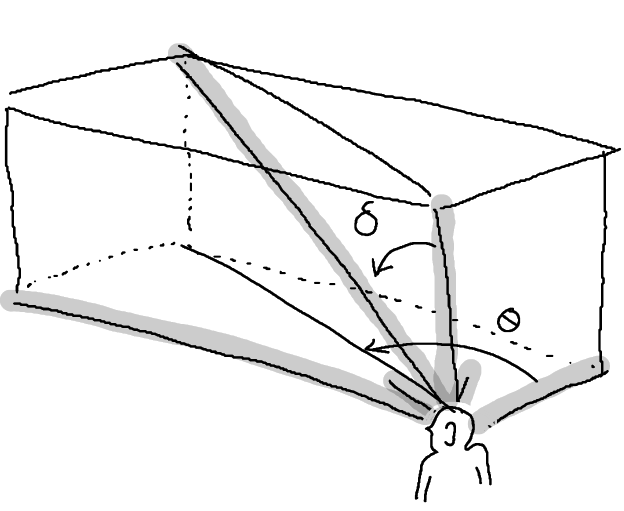
\includegraphics[keepaspectratio,scale=1]{04_att/direction.png}
\label{fig:}
\end{table}

\newpage

\begin{figure}[htbp]
    \centering
    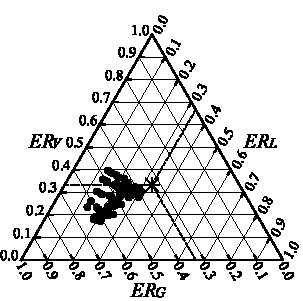
\includegraphics[keepaspectratio,scale=1.2]{05_att/rec_Ternary_out_14m.pdf}
    \caption{\hspace{1mm}Balance of three directional energy ratios of $H$=14[m]}
    \label{fig:sankaku14}
\end{figure}

\begin{figure}[htbp]
    \centering
    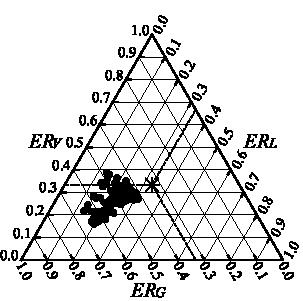
\includegraphics[keepaspectratio,scale=1.2]{05_att/rec_Ternary_out_12m.pdf}
    \caption{\hspace{1mm}Balance of three directional energy ratios of $H$=12[m]}
    \label{fig:sankaku12}
\end{figure}

\begin{figure}[htbp]
    \centering
    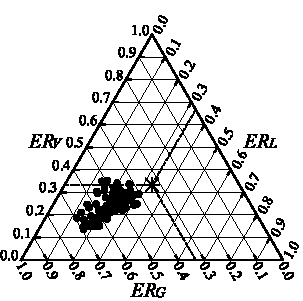
\includegraphics[keepaspectratio,scale=1.2]{05_att/rec_Ternary_out_10m.pdf}
    \caption{\hspace{1mm}Balance of three directional energy ratios of $H$=10[m]}
    \label{fig:sankaku10}
\end{figure}

\begin{figure}[htbp]
    \centering
    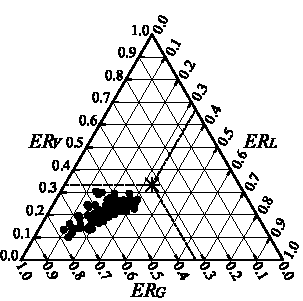
\includegraphics[keepaspectratio,scale=1.2]{05_att/rec_Ternary_out_8m.pdf}
    \caption{\hspace{1mm}Balance of three directional energy ratios of $H$=8[m]}
    \label{fig:sankaku8}
\end{figure}

\begin{figure}[htbp]
    \centering
    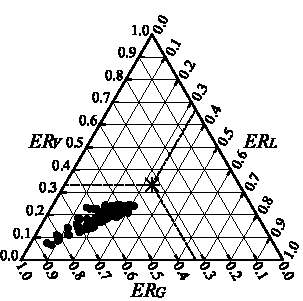
\includegraphics[keepaspectratio,scale=1.2]{05_att/rec_Ternary_out_6m.pdf}
    \caption{\hspace{1mm}Balance of three directional energy ratios of $H$=6[m]}
    \label{fig:sankaku6}
\end{figure}

\begin{figure}[htbp]
    \centering
    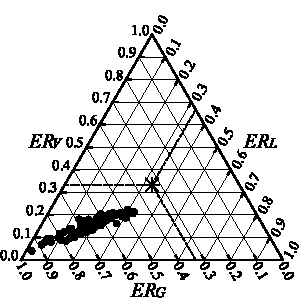
\includegraphics[keepaspectratio,scale=1.2]{05_att/rec_Ternary_out_4m.pdf}
    \caption{\hspace{1mm}Balance of three directional energy ratios of $H$=4[m]}
    \label{fig:sankaku4}
\end{figure}

\begin{figure}[htbp]
    \centering
    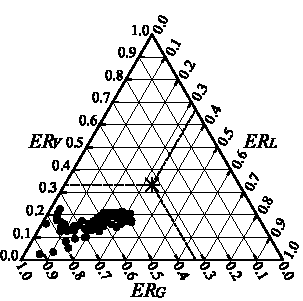
\includegraphics[keepaspectratio,scale=1.2]{05_att/rec_Ternary_out_2m.pdf}
    \caption{\hspace{1mm}Balance of three directional energy ratios of $H$=2[m]}
    \label{fig:sankaku2}
\end{figure}

\begin{figure}[htbp]
    \centering
    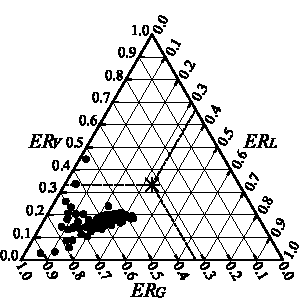
\includegraphics[keepaspectratio,scale=1.2]{05_att/rec_Ternary_out_1m.pdf}
    \caption{\hspace{1mm}Balance of three directional energy ratios of $H$=1.2[m]}
    \label{fig:sankaku1}
\end{figure}

\clearpage

\section{$DUI$の導入}
ここで鉛直方向・側方・前後方向から反射音エネルギが均等に到来するとき、$ER_V$、$ER_L$、$ER_G$の3値は全て$\frac{1}{3}$となることから、反射音の到来方向に関する空間バランスを見るための指標として3次元直交座標系における点($ER_V$,$ER_L$,$ER_G$)と点($\frac{1}{3}$,$\frac{1}{3}$,$\frac{1}{3}$)の距離$d_i$を観測点ごとに求め(\textbf{式}\ref{eq:di})、その空間内全観測点の平均値として$DUI$(Directional Uniformity Index)$^{\text{\cite{後期音}}}$を算出する(\textbf{式}\ref{eq:DUI})。$DUI$の空間分布を\figref{DUI_abs}に示す。

\begin{table}[htbp]
\begin{equation}
  \label{eq:di}
  d_i = \sqrt{\left({ER_V-\frac{1}{3}}\right)^2 + \left(ER_L-\frac{1}{3}\right)^2 + \left(ER_G-\frac{1}{3}\right)^2} 
\end{equation}
\begin{equation}
    \label{eq:DUI}
    DUI=\frac{\sum_{i=1}^N{d_i}}{N}
\end{equation}
\end{table}

\begin{figure}[p]
    \centering
    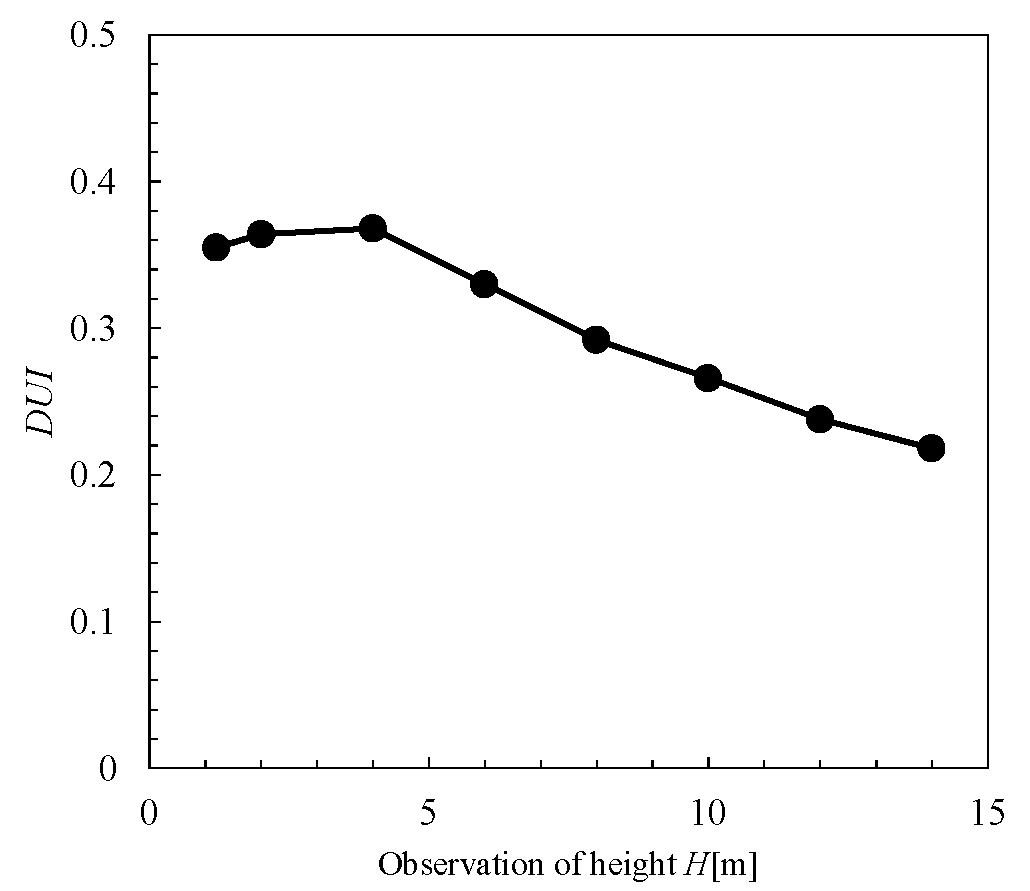
\includegraphics[keepaspectratio,scale=0.7]{05_att/DUI_abs2.pdf}
    \caption{\hspace{1mm}Spatial distribution of $DUI$}
    \label{fig:DUI_abs}
\end{figure}

\clearpage

\section{観測点の座標系について}
反射音方向分布特性をみるにあたり、観測点における座標系の置き方について2通りの検討を行った(\figref{observing})。\\
(i)観測点の座標系を解析モデルの3次元直交座標系にあわせる(正面:y軸負の方向)\\
(ii)観測点の座標系を音源中心の極座標系にする(正面:音源)\\
(i),(ii)それぞれの場合の$ER_V$、$ER_L$、$ER_G$及び$d_i$の分布を観測高さ$H$[m]ごとに示す。

\begin{figure}[htbp]
    \centering
    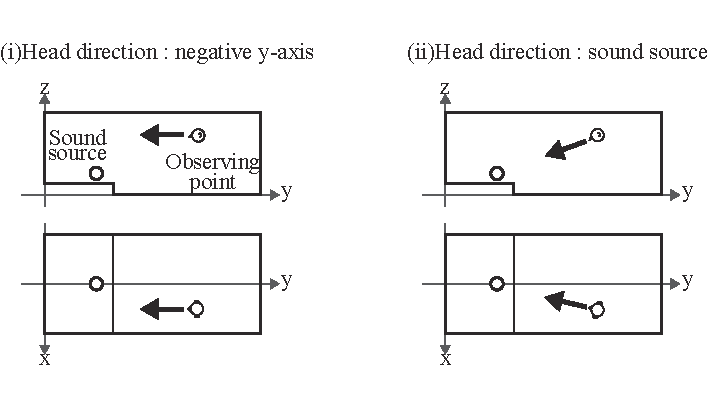
\includegraphics[keepaspectratio,scale=1]{05_att/observing.pdf}
    \caption{\hspace{1mm}\textbf{Study of head direction}}
    \label{fig:observing}
\end{figure}

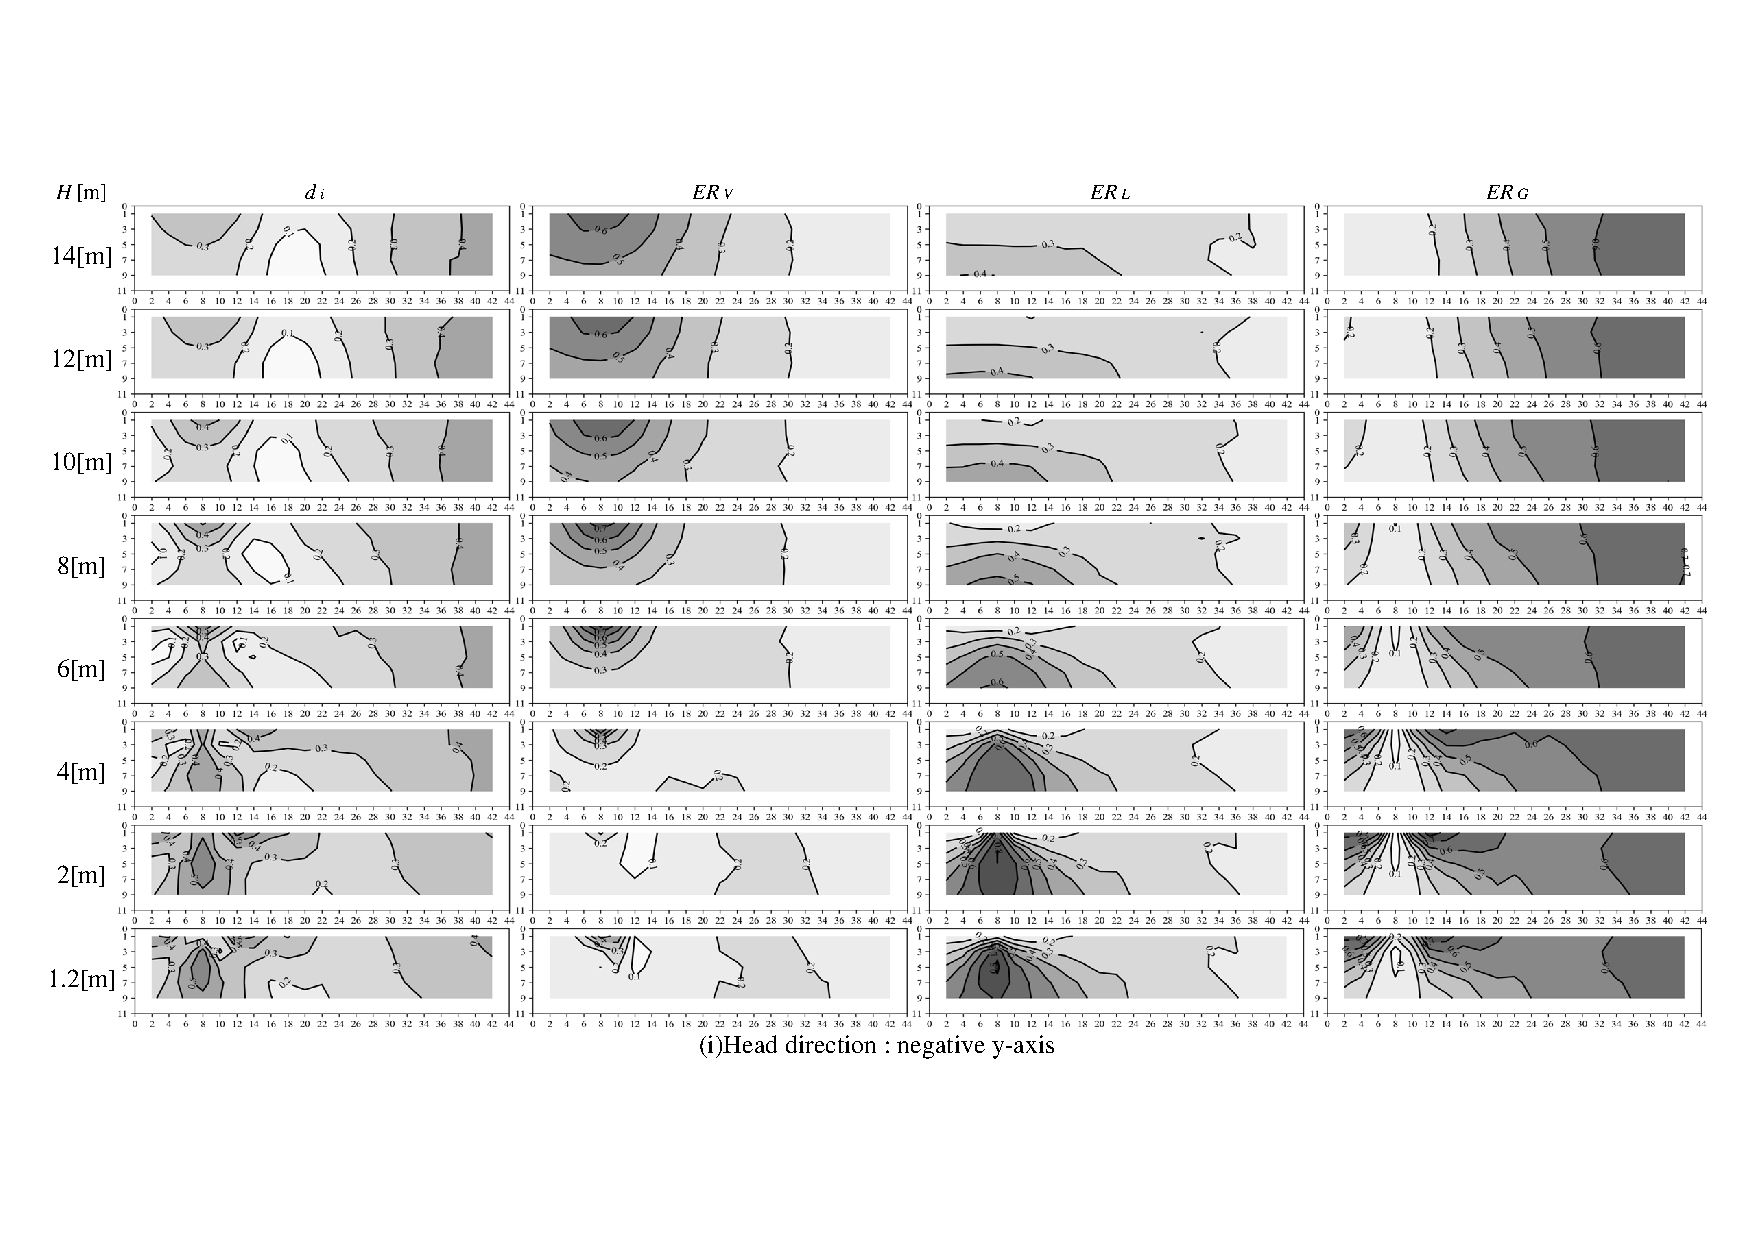
\includepdf[pages=-]{05_att/cont_y.pdf}
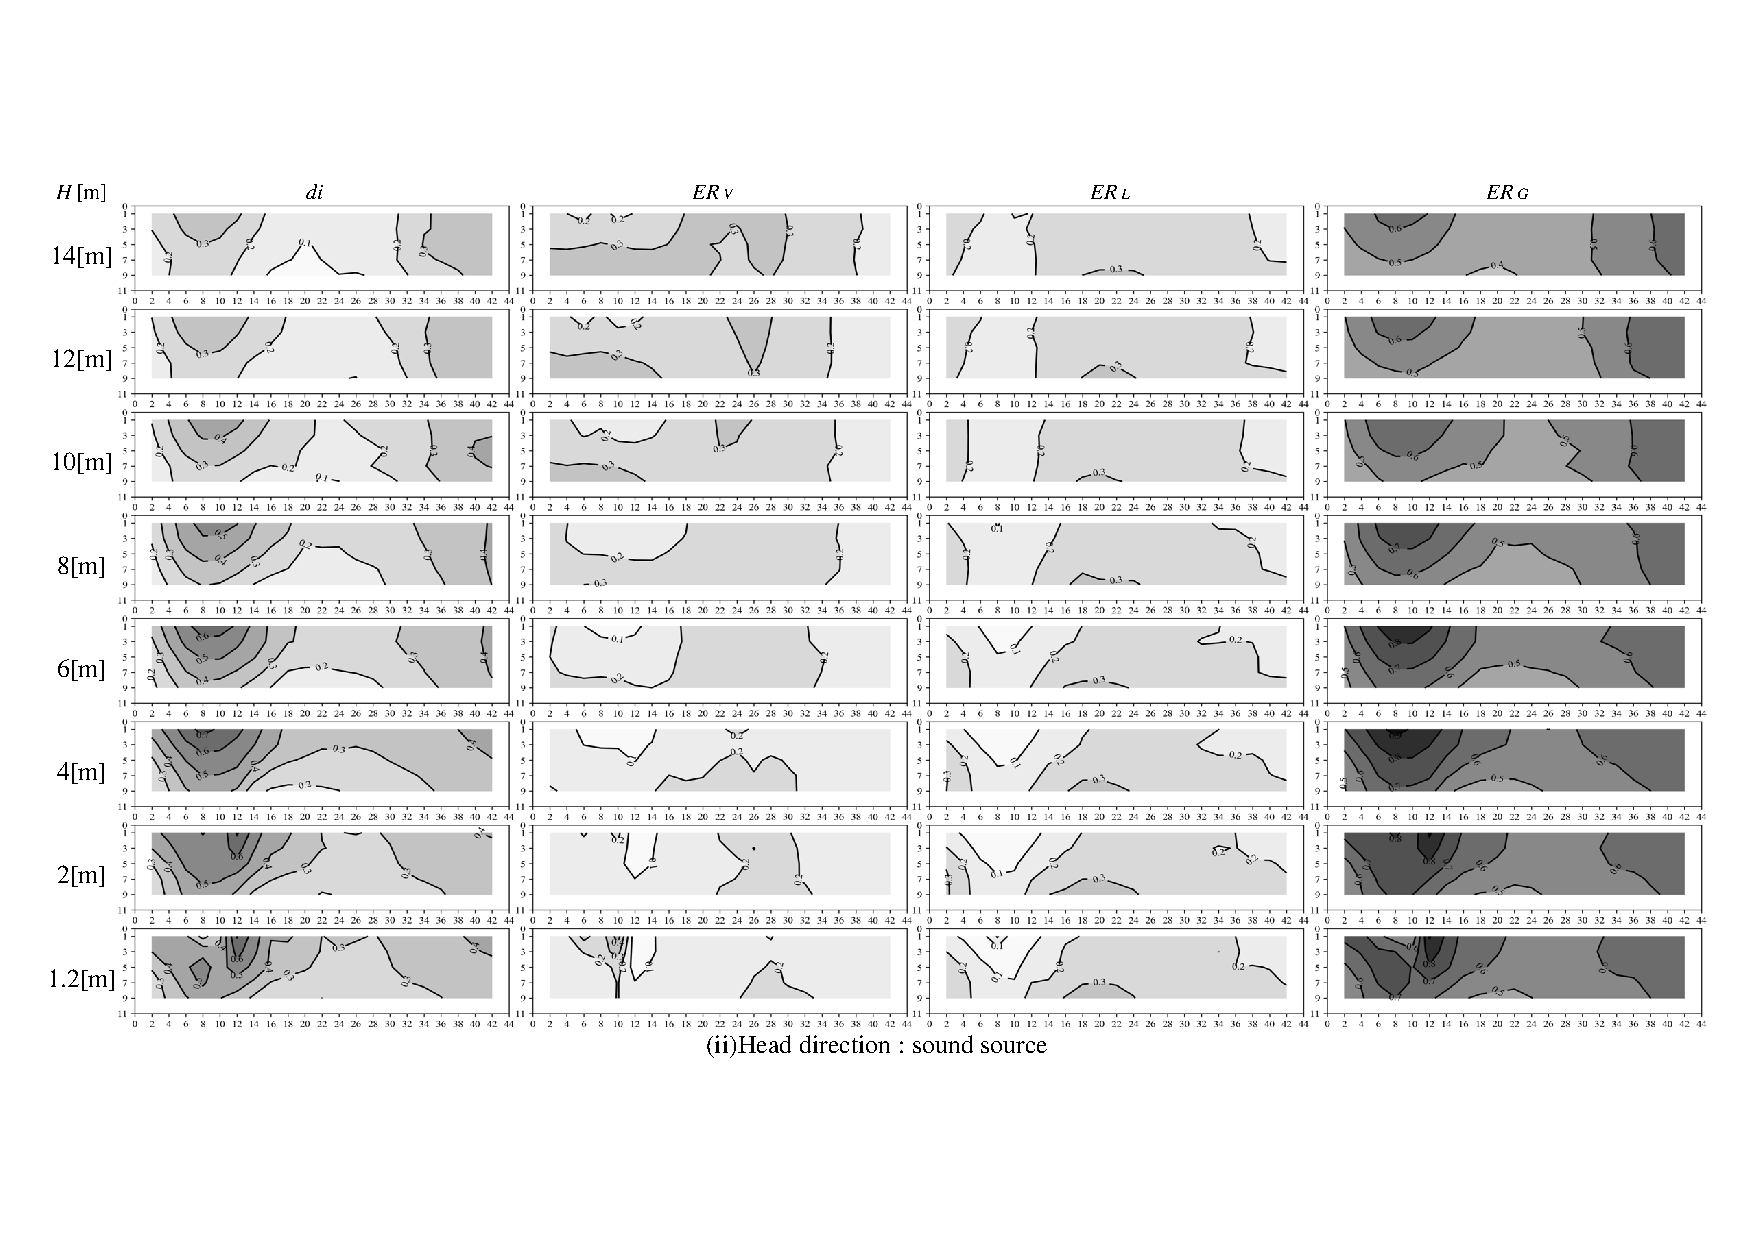
\includepdf[pages=-]{05_att/cont_s.pdf}

\subsubsection{(i)正面:y軸負の方向の場合}
天井付近では天井からの反射音が豊富に到来するが、座席部前方では前後方向成分が多くなり、座席後方では鉛直方向成分が多くなる。
すなわち、観測高さ$H$が高い音場では座席部前方で$ER_V$が、座席部後方で$ER_G$が大きな値をとっている(\figref{er_reason})。
一方、$ER_L$が音源付近で高い値をとっている。これは、頭の方向が常にy軸負の方向を向いているため、両耳方向に音源からの直接音が到来し、側方成分が多くなったと考えられる。
\\
\begin{figure}[htbp]
    \centering
    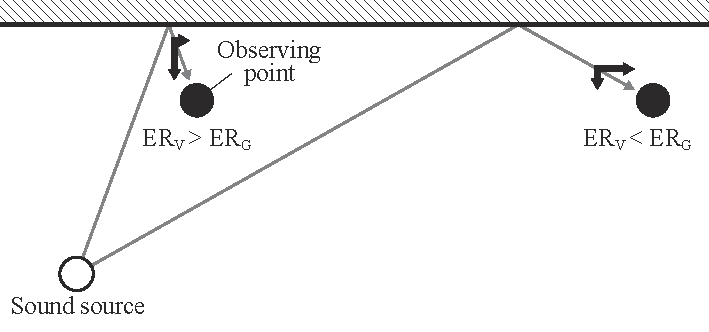
\includegraphics[keepaspectratio,scale=1]{05_att/er_reason.pdf}
    \caption{\hspace{1mm}\textbf{$ER_V$ vs $ER_G$}}
    \label{fig:er_reason}
\end{figure}

\subsubsection{(ii)正面:音源方向の場合}
常に頭が音源を向いているため、直接音は常に前後方向成分に含まれる。$ER_V$、$ER_L$、$ER_G$の和は常に1であるから、$ER_V$と$ER_L$に比べ$ER_G$が全体的に高い値をとっている。側壁付近で$ER_L$が高い値をとっているが、これは頭が音源を向いているため、両耳方向と側壁からの反射音の入射角が合うためであると考えられる。
\\ 本研究では実際にコンサートホールで音を聴いたときに受ける印象と反射音方向分布に符合する(ii)頭の向きを音源としたときの条件で解析を行う。

\pagebreak

\clearpage

\section{座席床面の吸音率が与える反射音方向分布への影響}
床面吸音率による影響をみるため座席床面を反射性としたモデルの解析を行った。
観測高さ$H$ごとの反射音方向別エネルギ比の分布を\figref{sankaku14_r}$\sim$\figref{sankaku1_r}に示す。
座席床面が反射性の場合においても観測高さが上がるにつれて分布が($\frac{1}{3}$,$\frac{1}{3}$,$\frac{1}{3}$)に集まる様子が確認できる。

\begin{figure}[H]
    \centering
    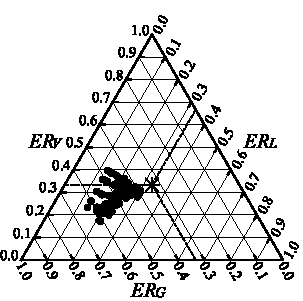
\includegraphics[keepaspectratio,scale=1.2]{05_att/reflect/rec_Ternary_out_14m.pdf}
    \caption{\hspace{1mm}Balance of three directional energy ratios of $H$=14[m]}
    \label{fig:sankaku14_r}
\end{figure}

\begin{figure}[H]
    \centering
    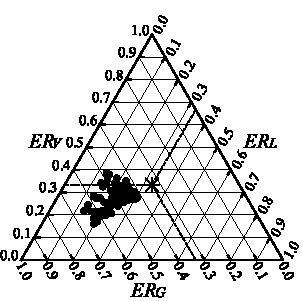
\includegraphics[keepaspectratio,scale=1.2]{05_att/reflect/rec_Ternary_out_12m.pdf}
    \caption{\hspace{1mm}Balance of three directional energy ratios of $H$=12[m]}
    \label{fig:sankaku12_r}
\end{figure}

\begin{figure}[H]
    \centering
    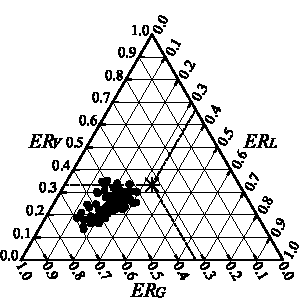
\includegraphics[keepaspectratio,scale=1.2]{05_att/reflect/rec_Ternary_out_10m.pdf}
    \caption{\hspace{1mm}Balance of three directional energy ratios of $H$=10[m]}
    \label{fig:sankaku10_r}
\end{figure}

\begin{figure}[H]
    \centering
    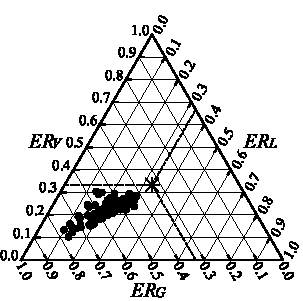
\includegraphics[keepaspectratio,scale=1.2]{05_att/reflect/rec_Ternary_out_8m.pdf}
    \caption{\hspace{1mm}Balance of three directional energy ratios of $H$=8[m]}
    \label{fig:sankaku8_r}
\end{figure}

\begin{figure}[H]
    \centering
    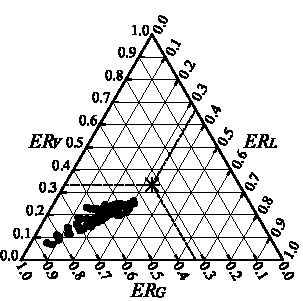
\includegraphics[keepaspectratio,scale=1.2]{05_att/reflect/rec_Ternary_out_6m.pdf}
    \caption{\hspace{1mm}Balance of three directional energy ratios of $H$=6[m]}
    \label{fig:sankaku6_r}
\end{figure}

\begin{figure}[H]
    \centering
    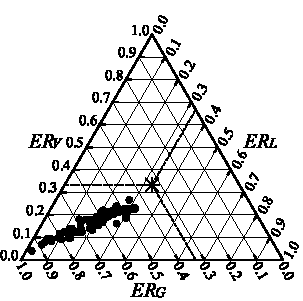
\includegraphics[keepaspectratio,scale=1.2]{05_att/reflect/rec_Ternary_out_4m.pdf}
    \caption{\hspace{1mm}Balance of three directional energy ratios of $H$=4[m]}
    \label{fig:sankaku4_r}
\end{figure}

\begin{figure}[H]
    \centering
    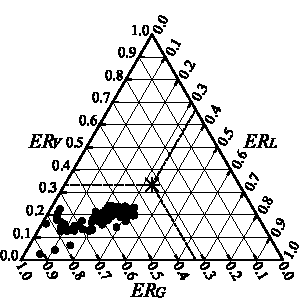
\includegraphics[keepaspectratio,scale=1.2]{05_att/reflect/rec_Ternary_out_2m.pdf}
    \caption{\hspace{1mm}Balance of three directional energy ratios of $H$=2[m]}
    \label{fig:sankaku2_r}
\end{figure}

\begin{figure}[H]
    \centering
    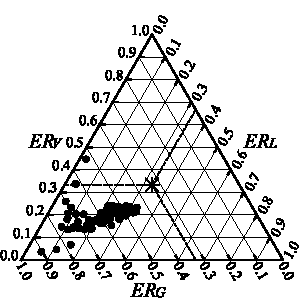
\includegraphics[keepaspectratio,scale=1.2]{05_att/reflect/rec_Ternary_out_1m.pdf}
    \caption{\hspace{1mm}Balance of three directional energy ratios of $H$=1.2[m]}
    \label{fig:sankaku1_r}
\end{figure}

座席床面が吸音性のモデルと座席床面が反射性のモデルにおける空間全体の$DUI$を比較したところ、吸音性は0.29、反射性は0.30であった。座席床面反射性のモデルにおける$DUI$の方が吸音性比べ0.01だけ小さい値をとり、$t$検定よりその差は危険率1$\%$で有意であった。また、両モデルの$DUI$を観測高さごとに比較すると、特に座席面近傍の反射音方向分布がより一様になることがわかる。\figref{DUI_abs}\\
 以上より座席床面を反射性とすることで反射音方向分布がより一様となることが示された。
 
\begin{figure}[H]
    \centering
    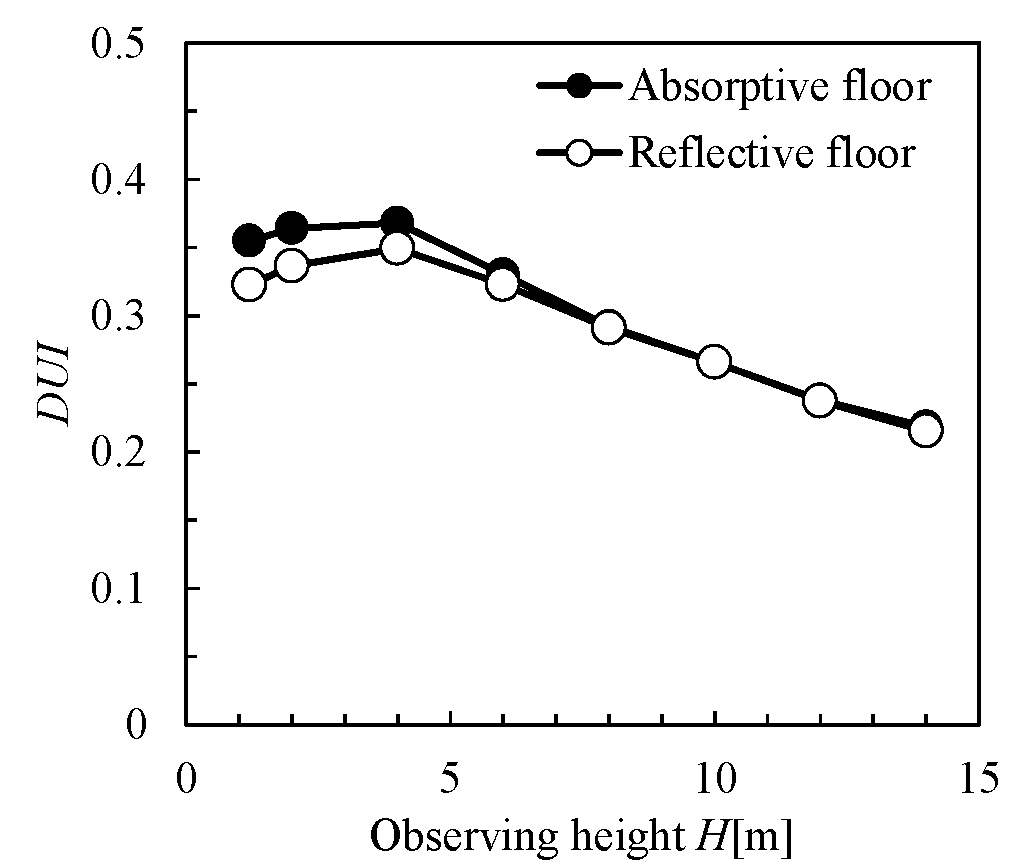
\includegraphics[keepaspectratio,scale=0.7]{05_att/reflect/DUI_ref2.pdf}
    \caption{\hspace{1mm}Spatial distribution of $DUI$}
    \label{fig:sankaku1_r}

\end{figure}